% !TEX root=/home/tavant/these/manuscript/src/manuscript.tex

\section{Canonical simulation result}
  \label{sec-canonical}
  
  
  The {\it canonical} case corresponds to the case when the walls are grounded, and are fully absorbing. 
  It is the reference case that will be extensively described and commented.
  Then, it will be used as reference to analyze and quantify the effects of two characteristics of the dielectric walls on the studied discharges : the secondary electron emission, and the modification of the electrostatic boundary condition.
  
  \subsection{Initial phase of the simulation: $t \leq 2\,\micro\second$} \label{subsec-initlaphase}
  
  The initial phase of the simulation corresponds to the growth of the \ac{ECDI}, and the formation of the sheaths.
  Because of the growth of the instability, the electron transport increases as well, that increases the electron heating.
  The time scale of the sheath formation is governed by the ion inertia.
  It is roughly the same time scale as the saturation of the instability due to ion-trapping.
  
  \begin{figure}[hbt]
    \centering
    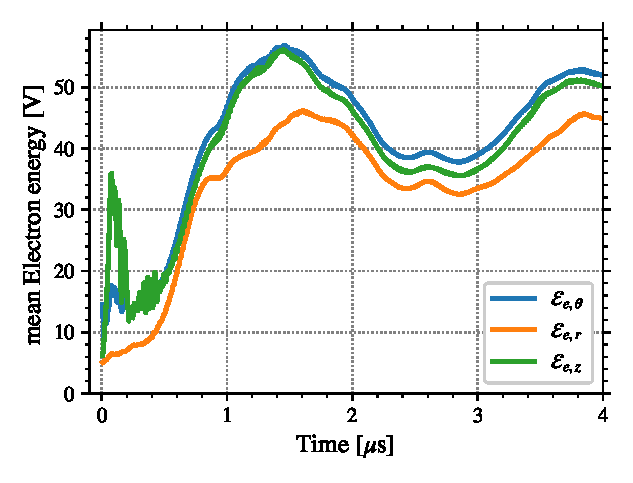
\includegraphics[width=\defaultwidth]{canonical_Te_start_directions}
    \caption{Temporal evolution of the electron mean kinetic energy decomposed over the three directions. Only the beginning of the simulation is shown.}
    \label{fig-canon_Te_strat}
  \end{figure}
  
  \Cref{fig-canon_Te_strat} shows the temporal evolution of the electron mean kinetic energy decomposed over the three directions, $\Ee_r, \Ee_{\theta}, \Ee_z$, such that
  \begin{equation} \label{eq-Ee_direction}
    \Ee_d = \frac{1}{n} \frac{1}{2} m_e \iiint_{\vect{v}}  v_{e,d}^2 f (\vect{v}) d^3v, \text{ with } d \in \{r, \theta, z  \}
  \end{equation}
  The mean kinetic energy is the sum of the thermal energy and the kinetic energy of the mean velocity.
  Because the electrons drift mainly in the azimuthal direction, we have
  \begin{equation} \label{eq-kinetic}
    \begin{cases}
      \Ee_r \simeq \frac{\Te_r}{2} \\
      \Ee_z \simeq \frac{\Te_z}{2} \\
      \Ee_{\theta} \simeq \frac{\Te_{\theta}}{2} + \frac{m_e}{2} \lp \frac{E_0}{B_0} \rp^2 \\
    \end{cases}
  \end{equation} 
  with $\frac{m_e}{2} \lp \frac{E_0}{B_0} \rp^2 \simeq  2.84\,\volt $.
  \nomenclature[Q]{\ensuremath{ \Ee}}{ Electron total kinetic energy, imposed of the thermal (or internal) energy and the kinetic energy of the mean velocity.  }
  We see that after some high frequency oscillations of $\Ee_{\theta}$ and $\Ee_z$ due to the cyclotron motion, the temperature rises before stabilizing at $\Ee \simeq 45$V.
  The radial kinetic energy $\Ee_r$ is less than $\Ee_z$ and $\Ee_{\theta}$, but only by a small difference of $5\,\volt$, corresponding to roughly $10\%$.
  The small difference between the azimuthal and the axial kinetic energy is of the order of $2\,\volt$, as expected from the cyclotron motion of the electrons and \cref{eq-kinetic}.
  This means that the electrons are almost isotropic.
  
  
  \begin{figure}[hbt]
    \centering
    \begin{tabular}{@{} c c}
      \subfigure{time_r_mean_n}{a}{20, 20} &
          
      \subfigure{time_r_mean_phi}{b}{20, 20} 
    \end{tabular}
    \caption{Temporal evolution of the radial profile of the ({\bf a}) electron density and ({\bf b}) the plasma potential averaged azimuthally.}
    \label{fig-tx_n_phi}
  \end{figure}

  We can see on \Cref{fig-tx_n_phi} the evolution of the radial profile of the electron density on the plasma potential over the same period as \cref{fig-canon_Te_strat}.
  We observe on both quantities the formation of the sheath and the evolution toward a steady-state.
  
  \subsection{Stable phase of the simulation\string: $t \geq 2\,\micro\second$}
  \label{subsec-stablephase}
  After the relatively fast rise of the plasma characteristics, the simulation stabilises at a steady-state, as we can see in \Cref{fig-canon_Te_all}.
  We observe that after $t\simeq2\mus$ , the electron energy $\Ee$ starts to oscillate around a mean value.
  The oscillations are then damped and reach their minimum amplitude at  $t\simeq 7\mus$ and then remain with a small amplitude as shown on simulations carried out up to $25\,\micro\second$ on \cref{fig-canon_Te_all}.
  Hence, there is no need to simulate for longer times than $10\mus$ in the following simulations.
  
  The origin of these oscillations is discussed in \Cref{subsec-temp}.
  
  
  \begin{figure}[hbt]
    \centering
    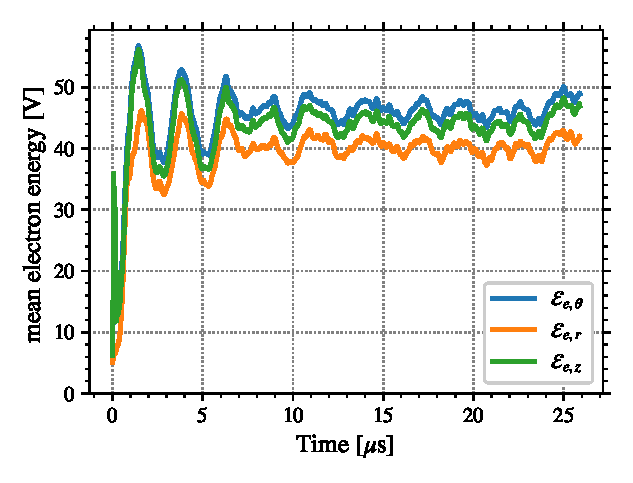
\includegraphics[width=\defaultwidth]{canonical_Te_all_directions_long}
    \caption{Temporal evolution of the electron mean kinetic energy decomposed over the three directions, similar to \cref{fig-canon_Te_strat} but for a longer period. We still see the difference between $\Ee_z$ and $\Ee_{\theta}$ due to the $E\times B$ drift, and the colder radial energy.}
    \label{fig-canon_Te_all}
  \end{figure}
  

  \Cref{fig-profiles} shows the azimuthally averaged radial profiles of the electron and ion densities  at steady-state.
  The plasma is mostly quasineutral, expect close to the walls.
  In the sheath, close to the wall, the electron density falls more rapidly compared to the ions.
  The sheath length can be roughly estimated to be $1\,\milli\meter$.
  The Debye length in our conditions is
  \begin{equation} \label{eq-debye}
    \lambda_D = \sqrt{\frac{\epsilon_0 k_b T_e}{n_e e^2}} \sim 0.4\,\milli\meter,
  \end{equation}
  which corresponds to the expected sheath length \citep{chabert2014}.
  
  \begin{figure}[hbt]
    \centering
    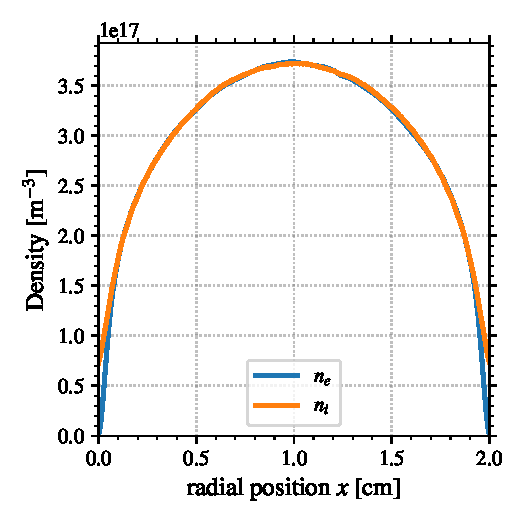
\includegraphics[width=\defaultwidth]{density_profile.pdf}
    \caption{Radial profile of the ion and electron densities at steady-state, averaged azimuthally and in time over the 5 last microseconds.}
    \label{fig-profiles}
  \end{figure}
  
  \subsection{Enhanced electron transport} \label{subsec-canonmue}
  As introduced in \cref{sec-transport}, the electron cross-field axial transport is characterized by the electron mobility
  \begin{equation} \label{eq-mobdef}
    \mob = \frac{u_{e, z}}{E_z}
  \end{equation}
  with $u_{e,z}$ and $E_z$ the electron mean axial velocity and the axial electric field, respectively.
  \nomenclature[Q]{\ensuremath{ \mob}}{ Electron mobility}
  \nomenclature[Q]{\ensuremath{ u}}{ Electron mean velocity}
  In \ac{PIC} simulations, $\mob$ is computed at each time step by
  \begin{equation} \label{eq-mobpic}
    \mobpic = \frac{1}{E_z} \sum_N v_{e,z}
  \end{equation}

  \begin{figure}[hbt]
    \centering
    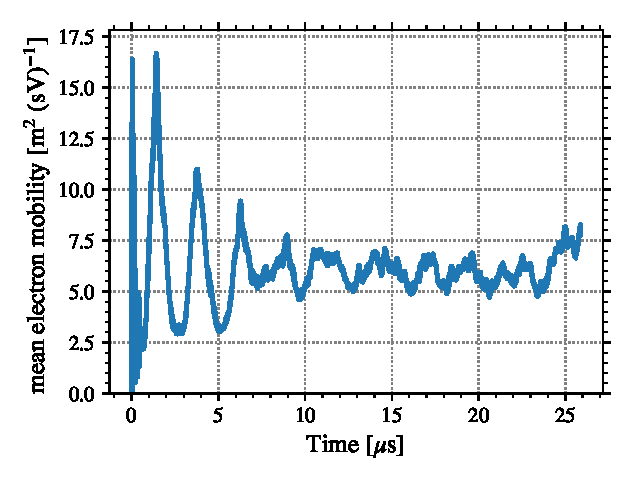
\includegraphics[width=\defaultwidth]{canonical_mu_all}
    \caption{Temporal evolution of the electron axial mobility computed in the \acs{PIC} simulation.}
    \label{fig-canon_mu}
  \end{figure}
  
  \Cref{fig-canon_mu} shows the temporal evolution of the electron mobility $\mobpic$ measured in the simulation with \cref{eq-mobpic}.
  We can see that it presents the same characteristics as the evolution of the electron energy $\Ee$ on \cref{fig-canon_Te_all}.
  We recall that the classical electron mobility from the collisional theory developed in \cref{eq-mobility} is \citep{lafleur2016a}
  \begin{equation} \label{eq-muclass}
    \mobcla = \frac{\nu_m \frac{e}{m_e}}{\oce^2 + \nu_m^2}
  \end{equation}
  with $\nu_m$ the electron-neutral  collision frequency and \oce is the electron cyclotron frequency.
  In the conditions of \cref{parameters}, $\mobcla \simeq 0.8$ \square\meter(sV)$^{-1}$.
  
  The measured electron mobility in the \ac{PIC} simulation is one order of magnitude larger than the classical mobility.
  In the present case, as no electron is emitted from the wall, the enhancement can only come from the instabilities present in the plasma, which induce an azimuthal electric field.

  % K_ex = 2 10^-13
  % n_g = 1e19
  % wce = q B / m
  The oscillations can be seen in \cref{fig-2dschemat}, which shows the azimuthal electric field observed at $T=4\,\micro\second$.
  It clearly features the oscillation of wavelength of the order of 1~mm, as observed in \citet{heron2013,janhunen2018}.
  \Cref{fig-exampleECDI} shows the temporal evolution of the azimuthal electric field measured at the center of the channel.
  We can see that the instability rises and saturates quickly.
  Then, the oscillation remains quite stable.
  The Fourier Transform of the electric field presents a clear maximum at $14\,\mega\hertz$.
  The theoretical frequency of the \ac{ECDI} instability is \citep{lafleur2017}
  \begin{equation} \label{eq-maxfeq}
    f_{\rm max} = \frac{\omega_{pi}}{\sqrt{3}} \simeq 21 \,\mega\hertz,
  \end{equation}
  which gives a relatively good agreement with the oscillation observed.
  The \ac{ECDI} instability was the subject of \Cref{ch-5}, hence it will not be further discussed here.
  
  
  \begin{figure}[hbt]
    \centering
    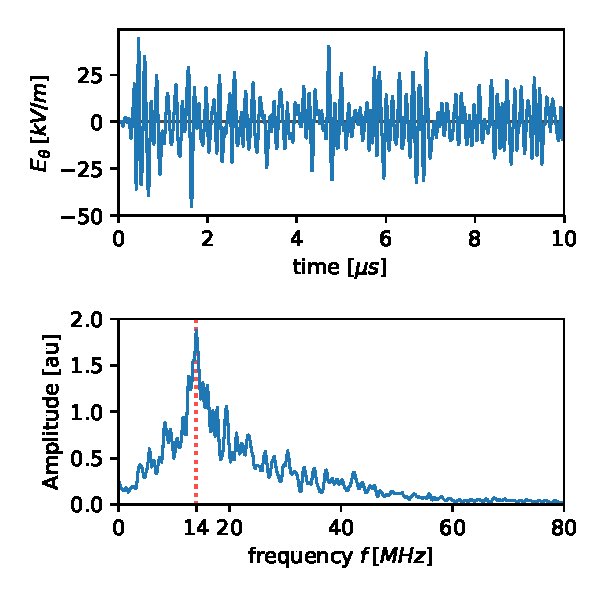
\includegraphics[width=\defaultwidth]{time_and_FFT}
    \caption{Azimuthal instability\string: temporal evolution of the azimuthal electric field at the center of the simulations, and its frequency spectra computed by \acs{FFT}. The frequency for which the amplitude is maximum is highlighted.}
    \label{fig-exampleECDI}
  \end{figure}
  
  we measure in the simulation the characters relative to the electron mobility.
  The effective mobility $\mobeff$ is determined by the correlation term $<\dEt \dne>$ and the parameters of the simulations.
  The effectively mobility at saturation $\mobeffsat$, using the hypothesis of saturation by ion-wave trapping, only need the electron temperature $\Te$.
  We can see that the three values $\mobpic, \mobeff$, and $\mobeffsat$ are close from each-others.
  
  \begin{table}[hbtp]
  \ra{1.3}
    \centering
    \caption{Characteristics relative to the electron mobility measured in the simulation at $t=27\,\micro\second$.}
    \label{tab-canonical_mobility}
    \begin{tabular}{@{} r l @{}} \toprule
    Quantity & Value \\ \midrule
    Correlation $<\dEt \dne>$ & $\sn{6}{20}$ V/m${^4}$ \\
    Effective mobility $\mobeff$ from \cref{eq-eq_mobeffsimple_two} & 4.4 m$^2$(sV)$^{-1}$ \\
    Mobility saturation $\mobeffsat$ from \cref{eq-mobeffsat} & 3.3 m$^2$(sV)$^{-1}$ \\
    Measured mobility $\mobpic$ from \cref{eq-mobpic} & 6 m$^2$(sV)$^{-1}$\\
    \bottomrule
    \end{tabular}
  \end{table}
  

  
  